\documentclass[12pt, letterpaper]{article}
\usepackage[utf8]{inputenc}
\usepackage[margin=1in]{geometry}
\usepackage{graphicx}
\usepackage{amsmath}
\usepackage{nccmath}
\usepackage{xcolor}

\pagecolor[rgb]{0.,0.,0.1}
\color[rgb]{1,1,1}

\graphicspath{ {./Chem 156 Images/} }

\setlength{\parskip}{1em}
\setlength{\parindent}{0em}


\begin{document}
    \section*{Chapter 14: Sedimentation Velocity}
    The external force (on a per molecule basis) due to centrifugation is 
    \textbf{m$\phi\omega^2$r}, where \boldmath{$\phi$} is the \textbf{density increment}
    , \textbf{$\omega$} is the \textbf{angular velocity}, m is the 
    \textbf{mass}, and r is the \textbf{radius}. The \textbf{opposing frictional force} is 
    \textbf{-fv}. When setting the sum of these forces to zero (terminal velocity), 
    the equation yields: 

    \begin{equation}
        V = \frac{m\phi\omega^2 r}{f}
    \end{equation}

        or, on a per mole basis: 

    \begin{equation}
        V = \frac{M\phi\omega^2 r}{N_Af}
    \end{equation}

    How do you visualize velocity \textbf{v} in a velocity sedimentation experiment? If the
    sample begins with the macromolecule uniformly distributed (concentration is equal everywhere
    in tube), then when centrifugation begins, the \textbf{top region} (low r) of the sample will lose its 
    macromolecules.  

        
 
   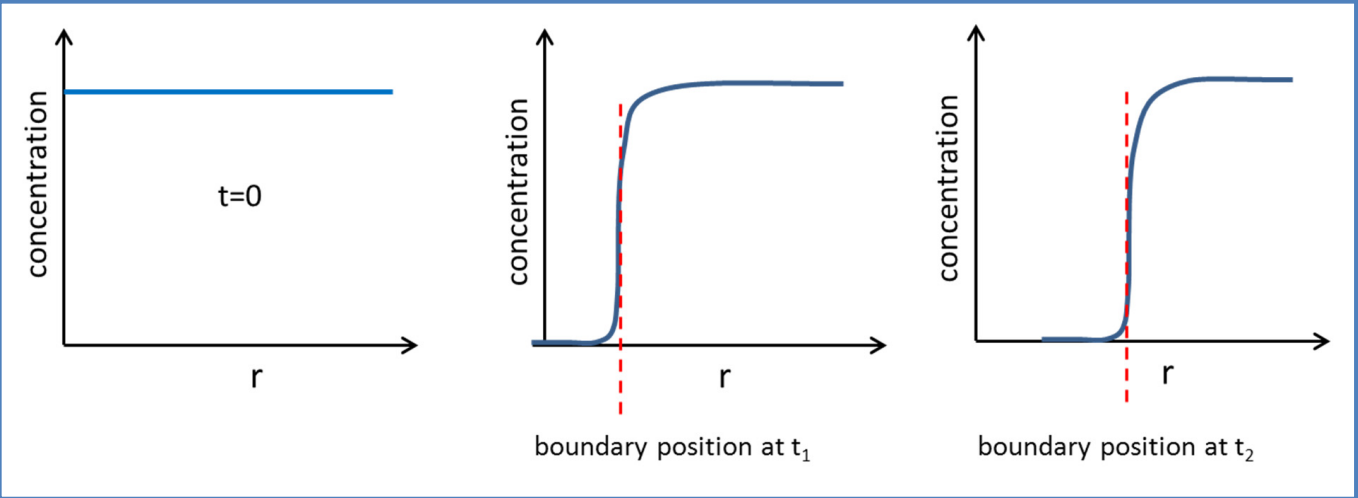
\includegraphics[scale = 0.70]{Sedimentaton Velocity with Radius.png}

    The sedimentation velocity $\textbf{v}$ is the speed of the boundary: \(\frac{\Delta r}{\Delta t} \) % need to do inline math here
    \\
    \\
    \\
    \\

    \subsection*{Meaning and Measurement of Sedimentation Coefficient, s}

    How does the sedimentation velocity \textbf{v} relate to molecular properties? From the equation
    \(V = \frac{M\phi\omega^2 r}{N_Af}\), v is affected by both molecular properties (M) and experimental
    parameters $(\omega)$. We want to separate the two kinds of variables on different sides of the equation: 

    \begin{equation}
        \frac{v}{\omega^2 r} = \frac{m\phi}{f}
    \end{equation}


    Now, introduce \textbf{sedimentation coefficient s} to be equal to those quantities. s is obtained experimentally using \(s = \frac{v}{\omega^2 r} \)
    s is obtained using molecular properties through:
    \begin{equation}
        s = \frac{M\phi}{N_Af} \; \text{ or } \useshortskip s = \frac{m\phi}{f}
    \end{equation}

    If angular velocity $\omega$ $\uparrow$, then the sedimentation velocity v $\uparrow$ from eq. (1). But the sedimentation coefficient s
    is unaffected. We know this is true becuase from \textbf{equation 4}, we can relate s to molecular properties without reference to 
    experimental parameters. 
    
    Since v is defined as \( \frac{dr}{dt}\) we can determine that: \\
    \begin{equation}
        s = \frac{\frac{dr}{dt} }{\omega^2 r} = \frac{\frac{dln(r)}{dt}}{\omega^2}
    \end{equation}

    Measuring the position r of the boundary at a series of time points during the experiment and plotting them as 
    \textbf{ln(boundary position) vs. t}  should give a straight line with slope s$\omega^2$, which can be used to find s.

    A special unit is used to express the value of the sedimentation coefficient (natural units are seconds). 
    The \textbf{Svedberg, S} is defined as $10^{-13}$ sec. 

    \subsection*{Relating s to molecular properties}

    The sedimentation coefficient relates to molecular properties in two ways: 
    \begin{itemize}
        \item dependence on mass
        \item frictional coefficient f (which depends on size $\rightarrow$ mass)
    \end{itemize}

    Starting with \(s = \frac{m\phi}{f} \), where f = 6$\pi\eta$R $\rightarrow$ \(s = \frac{m\phi}{6\pi \eta R}\)

    But R relates to volume and mass according to \(V = \frac{4}{3} \pi R^3 \) $\rightarrow$ \(R = (\frac{3V}{4 \pi})^{\frac{1}{3}} \)

    Relate volume V to mass m by the density $\rightarrow$ m = V$\rho$ and substitute V for $\frac{m}{\rho}$

    \begin{align*}
        s &= \frac{m \phi}{6 \pi \eta (\frac{3m}{4 \pi \rho})^{\frac{1}{3}}} \\ \\
       s &= m^{\frac{2}{3}} (\frac{\phi}{6 \pi \eta}) (\frac{4 \pi \rho}{3})^{\frac{1}{3}}  \hbox{ or } s = (\frac{M}{N_A})^{\frac{2}{3}} (\frac{\phi}{6 \pi \eta})(\frac{4 \pi \rho}{3})^{\frac{1}{3}}
    \end{align*}

    Do larger molecules sediment move faster or slower than small molecules of equal density and similar shape? Centrifugal force on an object 
    is proportional to mass, but opposing force is only $\frac{1}{3}$ power of the mass. 
    
    So larger molecules move faster, according to $\frac{2}{3}$ power of their mass.

    \textbf{This assumes that the protein or molecule is nearly spherical since we used Stoke's Equation}. If 
    the molecule of interest is \textbf{non-spherical}, then it will have the same centrifugal force but $\uparrow$ frictional 
    force $\rightarrow$ $\downarrow$ sedimentation coefficient s. This will result in a lower estimation for molecular 
    weight. 

    \subsection*{Combining s and D (diffusion coefficient) to get molecular weight without a spherical assumption}

    We can eliminate the assumption of spherical shape if we have measured values for s and D together. Having both values 
    cancels frictional coefficient out. We know that \(f = \frac{K_B T}{D} \) and from equation (4), \(f = \frac{M \phi}{N_A s} \) 
    If we equate the two together: 

    \begin{align*}
        f = \frac{K_B T}{D} &= \frac{M \phi}{N_A s} \\ \\
        M &= (\frac{RT}{\phi})(\frac{s}{D})
    \end{align*}

    Molecular weight relates only to the ratio of s to D, shape is no longer considered (frictional coefficient). 
    
    \newpage
    The diffusion coefficient D can be obtained from the sedimentation experiment itself. Under ideal conditions without
    diffusion, the concentration profile at the boundary would be perfectly steep. At a position just before the boundary 
    layer, there will be no macromolecules. Right at the boundary layer, there will be a concentration of macromolecules
    that is the same all throughout the tube after that layer.  

    \begin{center}
        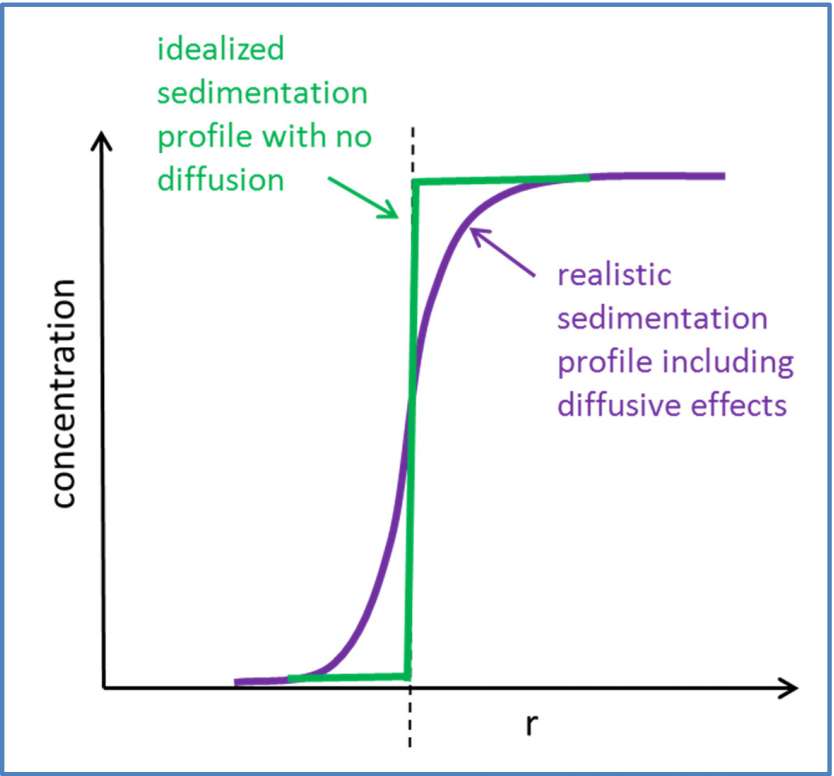
\includegraphics[scale = 0.70]{Sedimentation Profile.png}
    \end{center}

    \newpage

    \section*{Chapter 15: Chemical Reaction Kinetics}   
    \subsection*{Reaction Velocity, v}

    If we consider a reaction to be reactants $\rightarrow$ products, then reaction velocity v is the frequency
    (\#/time) wth which the event is occurring per unit volume. The units of v are \(\frac{\#}{volume \times time} \)
    or M/sec. There is only one velocity associated with the reaction, even though multiple reactants and products may be 
    involved. 

    The reaction velocity is indicated equally by the rate of change of \textbf{any} of the species involved:

    \begin{equation}
        \alpha A + \beta B + \dots \rightarrow \gamma C + \delta D + \dots
    \end{equation}
    \begin{align*}
        \frac{-d[A]}{dt} &= \alpha v \\
        \frac{-d[B]}{dt} &= \beta v \\
        \frac{d[C]}{dt} &= \gamma v \\
        \frac{d[D]}{dt} &= \delta v\\
    \end{align*}

    Rearranging to isolate velocity v gives \\
    
    \(v = - (\frac{1}{\alpha})(\frac{d[A]}{dt}) = (\frac{1}{\beta})(\frac{d[B]}{dt}) = (\frac{1}{\gamma})(\frac{d[C]}{dt}) = (\frac{1}{\delta})(\frac{d[D]}{dt}) = \dots \)
    
    Evidently, if we measure the rate of change of concentration of some species, then we measured reacton velocity v.

    \subsection*{Rate laws: how v depends on concentrations}
    Velocity of a reaction depends on how concentrated the reactants are. Besides concnetration, different reactions 
    (different chemical species) will have different v according to likelihood of underlying chemical events $\rightarrow$ k

    Combined dependence of v on rate constant k and concentrations $\rightarrow$ \textbf{rate law}. \\ \\

    Consider the equation: \(\mathrm{A} \stackrel{\mathrm{k}}{\longrightarrow} \mathrm{B} \)

    The rate law is \textbf{v = k[A]}, this reaction is first order in A. 

    Now consider \( 2\mathrm{A} \stackrel{\mathrm{k}}{\longrightarrow} \mathrm{B} \) $\Rightarrow$ \textbf{v = k[A]$^2$}, and the reaction is second order in A.
    


    If the equation is now \( \mathrm{A}+\mathrm{B} \stackrel{\mathrm{k}}{\longrightarrow} \mathrm{C} \), the rate law is now \textbf{v = k[A][B]}.

    \subsection*{Relationship of rate constants to equilibrium constants}

    What about if we had reversible processes? Velocities of forward and reverse reactions depend on the concentrations of 
    reactants and products, respectively. When the concentrations are reached where forward and reverse reactons are equal, 
    no \textbf{net} conversion is occurring. This is \textbf{chemical equilibrium}. Consider the reaction:

    \begin{equation}
        2 A \stackrel{k_1}{\underset{k_{-1}}{\rightleftharpoons}} B
    \end{equation}

    The \textbf{forward} reaction velocity is \textbf{v = k$_1$[A]$^2$} \\ \\
    The \textbf{reverse} reaction velocity is \textbf{v = k$_{-1}$[B]}


    At \textbf{equilibrium}, k$_1$[A]$^2$ = k$_{-1}$[B] and \( \frac{k_1}{k_{-1}} = \frac{[B]}{[A]^2} \)

    The ratio of the rate constants is equal to the equilibrium constant K. 

    \subsection*{Integrating Rate Laws}

    For simple reactions, we can integrate the differential equations that come from rate law to describe how concentrations of reactants and products change over time

    \underline{1st Order Decay}
    
    \(\mathrm{A} \stackrel{\mathrm{k}}{\longrightarrow} \mathrm{B} \)

    To get a differential equation in terms of [A], combine two points: 
    \begin{itemize}
        \item First need \(v = \frac{-d[A]}{dt} \)
        \item Also need \(v = k[A] \)
    \end{itemize}

    \newpage

    If we equate them together, we get the following: 

    \begin{align*}
        \frac{-d[A]}{dt} &= k[A] \\ \\
        \int \frac{d[A]}{[A]} &= -k \int dt \\ \\
        \ln[A] |_{[A]_0} ^{[A]} &= -\left.k t\right|_0 ^t 
    \end{align*}

    This gives us the familiar first order decay equations
    \begin{equation}
        \ln(\frac{[A]}{[A]_0}) = -kt
    \end{equation}

    \begin{figure}[h]
        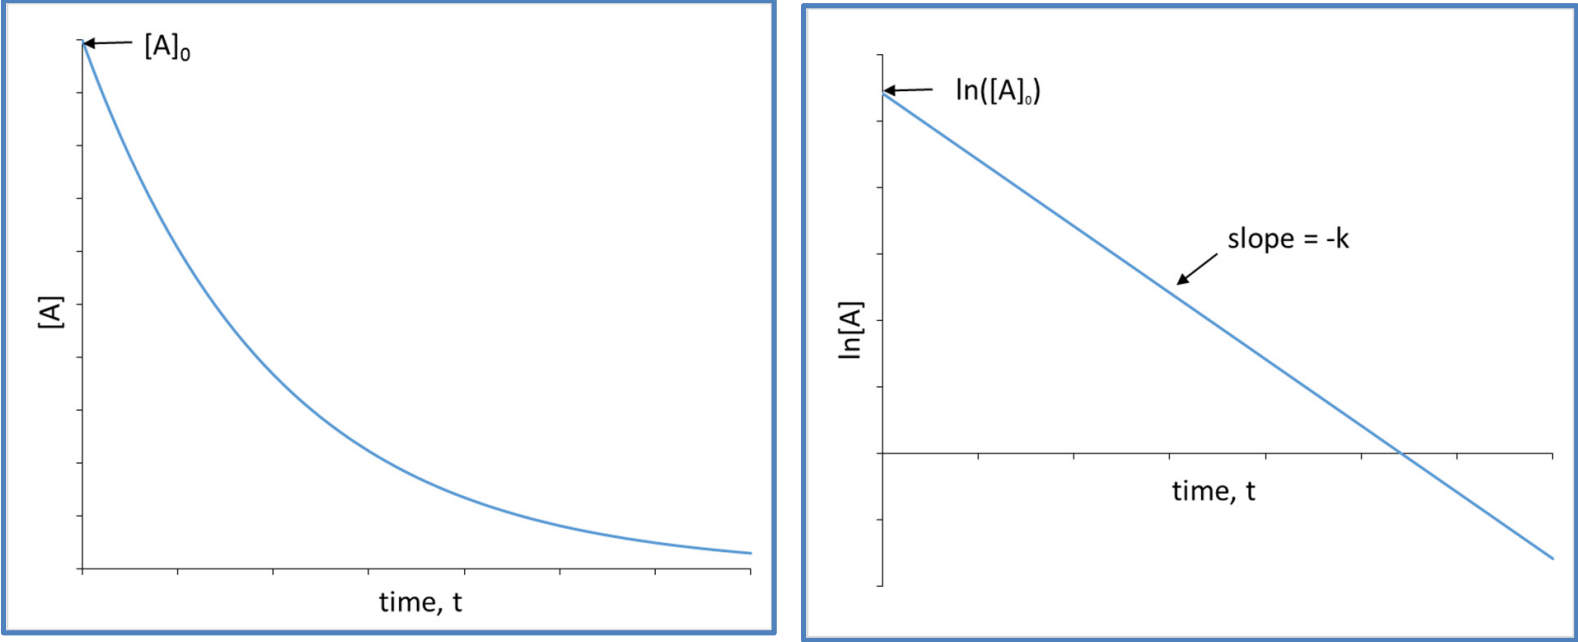
\includegraphics[scale = 0.6]{Reaction Rates.png}
        \caption{Behavior of [A] over time is exponential, while ln[A] is linear, with slope $\rightarrow$ k}
    \end{figure} 
    
    \underline{Describing decay times for 1st order decay}

    Time scale of first order decay is described in terms of half-life, $t_{1/2}$, which is the time required for a reaction to reach 50\% completion. 
    Parameter $\tau$ is used to describe decay times. It gives the time required for a reaction to reach $\frac{1}{e}$ completion compared to initial 
    condition: \( \frac{[A]}{[A]_0} = \frac{1}{e} \)

    \newpage

    We can connect $t_{1/2}$ and $\tau$ with the following comparison: 

    \begin{equation}
        \ln(\frac{1}{2})  = -kt_{\frac{1}{2}} \text{ to } \ln(\frac{1}{e}) = -1 = -k\tau
    \end{equation}

    This will give:

    \begin{equation}
        t_{\frac{1}{2}} = \ln(2) \tau
    \end{equation}

    For the simple first order decay reaction of [A] \\ \\
    \( t_{\frac{1}{2}} = \frac{\ln(2)}{k} \) and $\tau$ = $\frac{1}{k}$\\

    \underline{Integrated rate law for a 2nd order irreversible reaction}

    \(2\mathrm{A} \stackrel{\mathrm{k}}{\longrightarrow} \mathrm{B} \)

    Repeat the same process as above to get: 

    \begin{align*}
        \frac{-d[A]}{dt} &= 2k[A]^2 \\ \\
        \int \frac{d[A]}{[A]^2} &= -2k \int dt \\ \\
        -\frac{1}{[A]} |_{[A]_0} ^{[A]} &= -\left.2k t\right|_0 ^t \\ \\ 
        \frac{1}{[A]} - \frac{1}{[A]_0} &= 2kt
    \end{align*}
    
    A plot of $\frac{1}{[A]}$ vs. time gives a straight line, where slope = k

    \begin{center}
        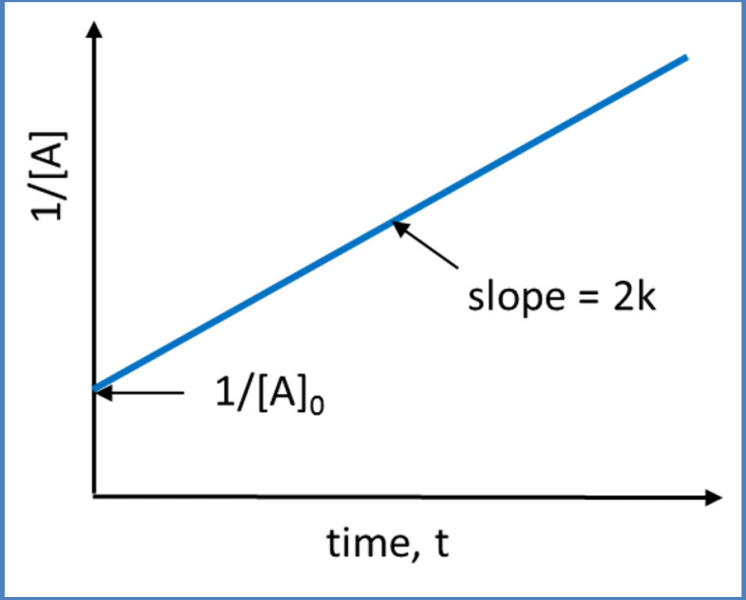
\includegraphics[scale = 0.35]{Rate Law Graph.png}
    \end{center}
    
    \subsection*{Establishing a rate law from measured reaction velocities}
    
    A different way of experimentally examining a rate law is by evaluating the 
    dependence of reaction velocity on concentrations. 

    If a reaction is \textbf{first order} in [A], then v will depend linearly on [A]. 
    If [A] doubles, then v will also double. 

    If a reaction is \textbf{second order} in [A], then doubling [A] will quadruple the 
    reaction velocity. 

    In general: 
    \begin{equation}
        v = [A]^{\alpha}
    \end{equation}

    Then for rate measurements made at two different concentrations: \\ \\
    \begin{equation}
        \ln(\frac{v_2}{v_1}) = \alpha \ln(\frac{[A]_2}{[A]_1})
    \end{equation}

    \subsection*{Behavior of more complex reaction schemes}

    Now, we want to consider events that are more complex than one step reactions. Consider 
    the following example: 

    \begin{equation*}
        A \stackrel{k_1} \longrightarrow B \stackrel {k_2} \longrightarrow  C
    \end{equation*}
   
    This gives the following equations:

    \begin{align*}
        \frac{d[A]}{dt} &= -k_1[A] \\ \\
        \frac{d[B]}{dt} &= k_1[A] - k_2[B] \\ \\
        \frac{d[C]}{[dt]} &= k_2[B]  
        %\frac{1}{[A]} - \frac{1}{[A]_0} &= 2kt
    \end{align*}
    
    \newpage
    For another example: 

    \begin{center}
        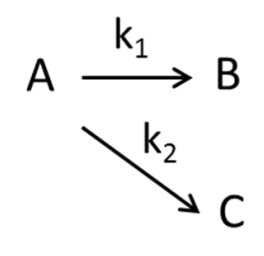
\includegraphics[scale = 0.5]{Complex Reaction.png}
    \end{center}

    The change in concentration as a function of time is given as: 

    \begin{align*}
        \frac{d[A]}{dt} &= -k_1[A] - k_2[A] = -(k_1 + k_2)[A] \\ \\
        \frac{d[B]}{dt} &= k_1[A] \\ \\
        \frac{d[C]}{[dt]} &= k_2[A]  
        %\frac{1}{[A]} - \frac{1}{[A]_0} &= 2kt
    \end{align*}

    \underline{Steady state assumptions for obtaining simple rate laws for complex reactions} \\ \\
    For complex reactions, dependence of the rate of the overall reaction (rate law) can depend on concentrations
    of species that do not contribue to the reaction itself.

    When sequential reactions are invovled, simplified rate laws can be obtained by assuming steady state conditions. 

    \textbf{Steady state} is when the intermediate species (that do not contribute to overall reaction stoichiometry) concentrations have reached
    constant value, at least momentarily.

    \begin{center}
        \( \frac{d[Intermediate]}{dt} = 0 \)
    \end{center}

    Consider the following equation: 
    \begin{equation}
        A \stackrel{k_1}{\underset{k_{-1}}{\rightleftharpoons}} B \stackrel{k_2} \longrightarrow C
    \end{equation}
    In this equation, the intermediate is B, and the overall reaction stoichiometry is \(A \longrightarrow C \).
    Based on equation 13, we can then state that: 

    \begin{align*}
        \frac{d[B]}{dt} &= k_1[A] - k_{-1}[B] - k_2[B] \\ \\
        &= k_1[A] - [B](k_{-1} + k_2) = 0
    \end{align*}

    Now rearrange to isolate [B]: 

    \begin{equation}
        [B] = \frac{k_1[A]}{k_2 + k_{-1}} 
    \end{equation}

    Now go back to the original reaction scheme. The overall reaction velocity is \( v = \frac{d[C]}{dt} \), but 
    we know that \( \frac{d[C]}{dt} = k_2[B] \). Substituting [B] from equation 14 shows that: 

    \begin{equation}
        v = \frac{k_1 k_2 [A]}{k_2 + k_{-1}}    
    \end{equation}

    From the equation 15 above, this 2-step reaction behaves as first order in [A] at steady state. 
   
    \subsection*{Enzyme Kinetics under a steady-state assumption}

    The following model is used to treat kinetics of a simple unimolecular enzyme reaction: 
    \begin{equation}
        E + S \stackrel{k_1}{\underset{k_{-1}}{\rightleftharpoons}} ES \stackrel{k_{cat}} \longrightarrow E + P
    \end{equation}

    E is the free enzyme, S is the free/unbound substrate, ES is the enzyme-substrate complex, and P is the product. 
    \( \frac{k_1}{k_{-1}} \) describes how the tightly the enzyme binds the substrate. $K_{cat}$ describes the catalytic rate 
    constant for formation of P. 

    The velocity of the overall reaction is described by \( v = \frac{d[P]}{t} \). According to the rate law, $v = k_{cat}[ES]$. 
    [ES] is an intermediate, and so we need to replace [ES] by adopting steady state assumption (where $\frac{d[ES]}{dt} = 0$).

    \begin{align*}
        \frac{d[ES]}{dt} &= k_1[E][S] - (k_{-1} + k_{cat})[ES] = 0 \\ \\
        [ES] &= \frac{k_1[E][S]}{k_{-1} + k{cat}}
    \end{align*}

    Now plug in [ES] from above into $v = k_{cat}[ES]$ : 

    \begin{equation}
        v =  \frac{k_{cat}k_1[E][S]}{k_{-1} + k_{cat}}
    \end{equation}

    This equation is a start, but it only describes the reaction velocity in terms of the free enzyme concnetration. 
    In an experiment, we usually only have control over the total enzyme concnetratoin. We want to rewrite the equation 
    in terms of total enzyme concentration and in terms of the ratio of the reaction velocity to the maximum possible value ($[ES] = [E]_{total}$)
    The maximum velocity is $k_{cat} \times \text{max value for } [ES]$, which is: 

    \begin{equation}
        v_{max} = k_{cat}[E]_{total} = k_{cat}([ES] + [E])
    \end{equation}
    The ratio of reaction velocities relative to its maximum is given: 

    \begin{align*}
        \frac{v}{V_{max}} &= \frac{k_{cat}[ES]}{k_{cat}([E] + [ES])} \\ \\
        \frac{v}{V_{max}} &= \frac{[ES]}{([ES] + [E])} \\ \\
        \frac{v}{V_{max}} &= \frac{1}{1 + \frac{[E]}{[ES]}}
    \end{align*}

    Taking the previous equation \( [ES] = \frac{k_1[E][S]}{k_{-1} +  k_{cat}} \) and rearranging so that \\ it becomes \( \frac{[E]}{[ES]} = \frac{k_{-1} + k_{cat}}{k_1[S]}\), substitute this equation above to give:

    \begin{align*}
        \frac{v}{V_{max}} &= \frac{1}{1 + \frac{k_{-1} + k_{cat}}{k_1[S]}} \\ \\
        \frac{v}{V_{max}} &= \frac{[S]}{[S] + \frac{k_{-1} + k_{cat}}{k_1[S]}} \\ \\
        \frac{v}{V_{max}} &= \frac{[S]}{[S] + K_M} \longrightarrow K_M = \frac{k_{-1} + k_{cat}}{k_1}
    \end{align*}
    
    Or, we can also convert from fractional velocity to v using equation 18 for $V_{max}$:

    \begin{equation}
        v = \frac{k_{cat}[E]_{total}[S]}{[S] + K_M}
    \end{equation}

    \newpage

    \subsection*{Relaxation kinetics: how systems approach equilibrium}
    \subsubsection*{The T-Jump Method}
    The temperature jump method was developed to study fast reactions and their "relaxation" back towards equilibrium. 
    If energy is rapidly delivered to a solution containing reactant and product at equilibrium, the temperature of the 
    system can be heated nearly instantaneously. Recalling the \textbf{van't Hoff equation}, if $\Delta$H for the reaction is non-zero,
    then the equilibrium constant will be different at a new temperature. Then you can observe how fast the reaction returns to its 
    new equilibrium. 

    The speed at which equilbrium is achieved depends on the forward and backward rate constants of the reaction. 

    Consider a simple system:

    \begin{equation*}
        A \stackrel{k_1}{\underset{k_{-1}}{\rightleftharpoons}} B
    \end{equation*}

    Let $\textbf{x}$ be the distance of each species from equilibrium. $\bar{A}$ will be $[A]_{equilbrium}$ at the new temperature, same for $\bar{B}$.
    The concentrations of A and B are related to the equilibrium conc. by: 
    \begin{align*}
        [A] &= \bar{A} + x \\
        [B] &= \bar{B} - x
    \end{align*}
    
    Now examine the approach to equlibrium by writing an equation for time dependence of \textbf{x}. 

    \begin{align*}
        \frac{d[A]}{dt} &= \frac{d[\bar{A} + x]}{dt} = \frac{dx}{dt} \\ \\ 
        \frac{d[A]}{dt} &= -k_1[A] + k_{-1}[B] \\ \\
        \frac{d[A]}{dt} &= -k_1[\bar{A} + x] + k_{-1}[\bar{B} - x] \\ \\
        &= k_{-1}\bar{B} - k_{1}\bar{A} - x(k_1 + k_{-1})
    \end{align*}

    The term \(k_{-1}\bar{B} - k_{1}\bar{A} = 0 \) because \( \frac{\bar{B}}{\bar{A}} = K = \frac{k_1}{k_{-1}} \)

    So, after setting the above to 0, the equation yields: 

    \begin{equation}
        \frac{dx}{dt} = -(k_1 + k_{-1})x
    \end{equation}

    X follows first order kinetics. Skipping the familiar detials for handling a first order differential equation: 

    \begin{equation}
        x = x_o^{-(k_1 + k_{-1})} \text{ and } \ln(\frac{x}{x_0}) = -(k_1 + k_{-1})t
    \end{equation}

    Convert these to even more general forms:

    \begin{equation}
        x = x_0e^{\frac{-t}{\tau}} \text{ and } \ln(\frac{x}{x_0}) = \frac{-t}{\tau}
    \end{equation}
    
    where \( \tau = \frac{1}{k_1 + k_{-1}} \)

    \begin{center}
        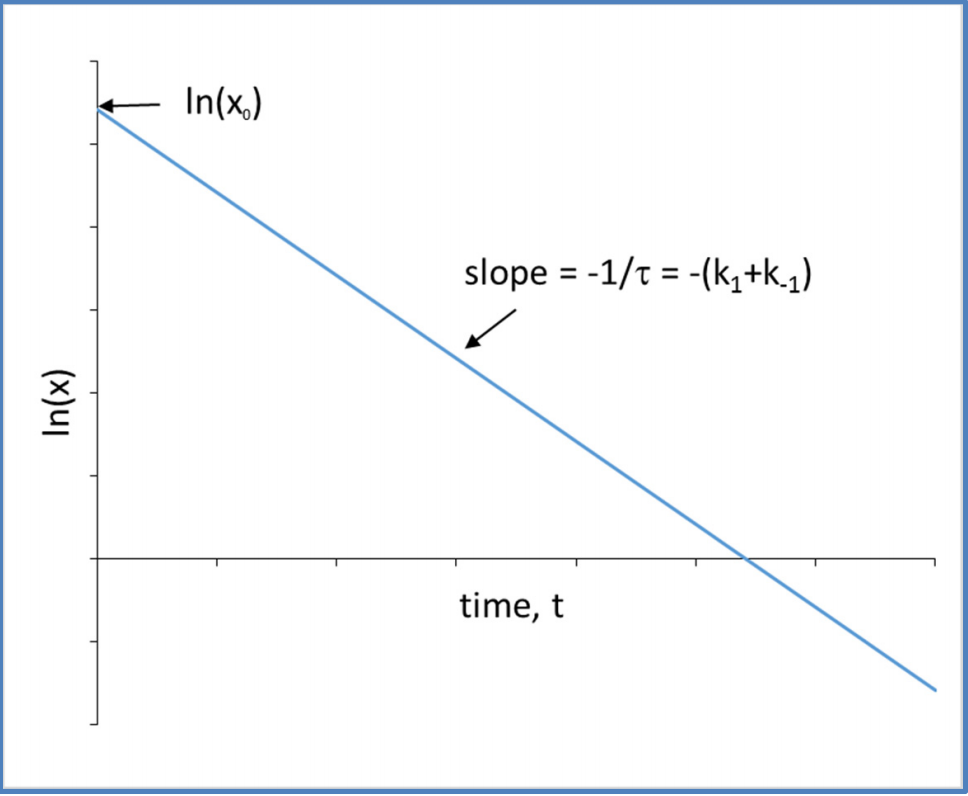
\includegraphics[scale = 0.4]{ln(x) vs. time.png}
    \end{center}
    
    If you can find [A] or [B] as a function of time, then you can also find \textbf{x} as a function of time. 

    \textbf{x} = $[A] - \bar{A}$ = $\bar{B} - [B]$

    You can use this to measure $\tau$, and thus also \(k_1 + k_{-1} \)

    \begin{align*}
        1/\tau &= k_1 + k_{-1} \text{ and } k_1 = Kk_{-1} \\ \\ 
        1/\tau &= Kk_{-1} + k_{-1} = (K+1)k_{-1}
    \end{align*}

    \begin{equation*}
        k_{-1} = \frac{1}{\tau(K + 1)} \text{ and } k_1 = \frac{K}{\tau(K + 1)}
    \end{equation*}

\subsubsection*{Higher Order Reactions Approaching Equilibrium}

Now consider this second order reversible reaction:

\begin{equation*}
    A + B \stackrel{k_1}{\underset{k_{-1}}{\rightleftharpoons}} C
\end{equation*}

There is only one transformation, so the distance can still be described by \textbf{x}:

\begin{align*}
    [A] &= \bar{A} + x \\ \\ 
    [B] &= \bar{B} + x \\ \\
    [C] &= \bar{C} - x
\end{align*}

We can use the same approach from the above to describe the change in concentrations: 

\begin{align*}
    \frac{d[A]}{dt} &= \frac{d(\bar{A} + x)}{dt} = \frac{dx}{dt} \\ \\
    \frac{d[A]}{dt} &= -k_1(\bar{A} + x)(\bar{B} + x) + k_{-1}(\bar{C} - x) \\ \\ 
    &= k_{-1}\bar{C} - k_1\bar{A}\bar{B} - x(k_1(\bar{A} + \bar{B}) + k_{-1}) - k_1x^2
\end{align*}

\( k_{-1}\bar{C} - k_1\bar{A}\bar{B} \) cancels to 0, and if we are close enough to equilibrium then x is small, so we can neglect the $x^2$ term. 
So, 

\begin{equation}
    \frac{dx}{dt} = -(k_1(\bar{A} + \bar{B}) + k_{-1})x
\end{equation}

So, the distance from equilibrium x shows first order behavior close to equilibrium, with \( \tau = \frac{1}{k_1(\bar{A} + \bar{B}) + k_{-1}} \)

\newpage

\subsection*{Kinetics from Single Molecule Studies}
For a unimolecular event, we can get a sense for the rate constant by looking at how long the molecule
persists in its current state before undergoing a reaction. 

Think of this as the "waiting time" before a reaction or confroational change occurs. 
While reactions are random, the average waiting time should be shorter for a process with a higher rate constant. 

Consider \( A \longrightarrow B \) with rate constant k. 

How long before any molecule A turns into B? Treat the reaction in bulk: 

\begin{equation}
    \frac{A}{A_0} = e^{\frac{-t}{\tau}} \text{ where } \tau = \frac{1}{k}
\end{equation}

$\frac{A}{A_0} $ can be considered the probability that any molecule A will \textbf{not} convert at time t. 

The probability that molecule A reacts precisely at time t is \( P(A)_{react} = \frac{1}{\tau} e^{\frac{-t}{\tau}} \).

To get the average time at which a molecule of A reacts (aka waiting time), we need
to get the average value of t by weighting all possible values of t by probability of reaction at time t. 

\textbf{To do this}, multiply t by the probability of reaction at time t, then integrate from t = 0 to infinity. 

\begin{equation}
    \text{waiting time} = \int_{t = 0}^{t = \infty}(t(\frac{1}{\tau})e^{\frac{-t}{\tau}})dt
\end{equation}

If we can measure how long it takes a single molecule to undergo a transition,then we have measured $\tau$. 

\newpage

\section*{Chapter 16: Kinetic Theories and Enzyme Catalysis}
Now we want to look at what determines the rate constant, k. What makes some reactions innately fast or slow?
There are two main models that try to explain the mechanisms of chemical reactions and their rate constants. 

\subsection*{The Arrhenius Equation}

This is often used to discuss reaction rates in terms of \textbf{molecular collisions}. 
The rate constant k is determined by:

\begin{equation}
    k = Ae^{-\frac{E_a}{RT}}
\end{equation}

A is the \textbf{frequency factor} and $E_a$ is an \textbf{activation energy}. 
We already know that the frequency of collisions in a reaction is dependent on concentrations. 
The frequency factor in the equation for k accounts for other phenomena ie. the dependence of molecular
velocities and consequently collision rates on temperature, and the dependence of reaction probability on 
the orientation of the colliding molecules. 

\textbf{$E_a$} describes a lower bound for energy that reactants must have for reaction to occur. Why does $E_a$ 
enter the equation for k as an exponential term? \textbf{Boltzmann Distrbution!}

If \( N(E) \propto e^{\frac{-E}{RT}} \), then we can find the fraction of molecules having energy at least as high as $E_a$ by 
\textbf{taking the ratio of area that falls under the curve and has E $\geq$ $E_a$} divided by entire area under the curve. 

\begin{align*}
    \frac{\int_{E_a}^{\infty}  e^{\frac{-E}{RT}}}{\int_{0}^{\infty}  e^{\frac{-E}{RT}}} &= \frac{-RTe^{\frac{-E}{RT}} |_{E_a}^{\infty}}{-RTe^{\frac{-E}{RT}}|_{0}^{\infty}} \\ \\
    \frac{e^{-\frac{E_a}{RT}}}{1} &= e^{-\frac{E_a}{RT}}
\end{align*}

A key element of Arrhenius equation: \textbf{the rate constant depends strongly on the height of an energy barrier.} 
It also depends on the temperature.

\newpage
The dependence of k on T can be used to evaluate the activaton energy in the Arrhenius model. 

\begin{equation*}
    \frac{d(ln(k))}{dt} \cong \frac{d(\frac{-E_a}{RT})}{dT} = \frac{E_a}{RT^2}
\end{equation*}
or 

\begin{align*}
    \frac{d(ln(k))}{d(\frac{1}{T})} \cong \frac{d(\frac{-E_a}{RT})}{d(\frac{1}{T})} &= \frac{d(\frac{-E_a}{RT})}{-\frac{d(T)}{T^2}} \\ \\ 
    &= \frac{-E_a}{RT^2} = \frac{-E_a}{R}
\end{align*}

\subsection*{Eyring Transition State Theory}
This method provides a slightly different way of looking at things that are more explicit about the occurrence of high energy species during 
a single reaction event. A single reaction step: 

\begin{equation}
    A + B \stackrel{k} \longrightarrow C
\end{equation}

is broken down in terms of two steps. 
\begin{itemize}
    \item First step: unstable high energy species (the transition state)
    \item Second step: the transition breaks down to product. 
\end{itemize}

The double-dagger symbol indicates the \textbf{transition state}. 
\begin{equation*}
    A + B \stackrel{k_{+ \ddagger }}{\underset{k_{- \ddagger}}{\rightleftharpoons}} AB^{\ddagger} \stackrel{k_{breakdown}} \longrightarrow C
\end{equation*}

The rate constant for breakdown of transition state is approximately 
the frequency of molecular vibrations, which is on the order of \textbf{$\frac{k_BT}{h}$}, where \emph{h} is \textbf{Planck's Constant}

\begin{equation}
    k_{breakdown} = \frac{k_BT}{h} \text{ and } v = \frac{d[C]}{dt} = k_{breakdown}[AB\ddagger]
\end{equation}
Then, the velocity of the reaction scheme above is: 

\begin{equation}
    v = \frac{d[C]}{dt} = \frac{k_BT}{h}[AB^{\ddagger}]
\end{equation}
\newpage

If we assume that the first step (formation of the transition state) is at 
equilibrium, then \( \frac{k_+ \ddagger}{k_- \ddagger} = K\ddagger = \frac{[AB\ddagger]}{[A][B]} \),
so, \( [AB\ddagger] = K\ddagger[A][B] \). If we substitute this value, 
then the reaction velocity would be \( v = \frac{k_BT}{h}K\ddagger[A][B] \)

Match this up to the simple rate law we would write for a single
elementary reaction \( \rightarrow v = k[A][B] \). The Eyring Model 
gives: 

\begin{equation*}
    k = \frac{k_BT}{h}K\ddagger
\end{equation*}

The rate constant \emph{k} is largely dependent on the equilibrum constant $K\ddagger$ for forming
the transition state. We can also write $K\ddagger$ in terms of free energy for reaching the transition state: 

\begin{equation*}
    K\ddagger = e^{\frac{- \Delta G}{RT}}
\end{equation*}

Substituting this gives us the equation: 

\begin{equation}
    k = \frac{k_BT}{h}e^{\frac{- \Delta G}{RT}}
\end{equation}

While this is different than the \textbf{Arrhenius Equation}, it is similar in that 
it shows the exponential dependence on an energy barrier.

We can also look at the temperature difference of ln(k) for the Eyring equation like we did for the Arrenhius:

\begin{align*}
    \frac{d\ln(k)}{dT} &\cong \frac{d(\frac{- \Delta G \ddagger}{RT})}{dT} \\ \\ 
    &= \frac{d(\frac{- \Delta H \ddagger}{RT} + \frac{\Delta S}{R})}{dT} \\ \\
    &= \frac{\Delta H \ddagger}{RT^2}
\end{align*}

The activation energy in the Arrhenius Equation relates closely to the transition state enthalpy in the Eyring model. 
\newpage

\subsection*{Catalysis by lowering the transition state energy}

The Eyring transition state model provides a way to look at catalysis in terms of transition state energies.

Let the rate constant for the uncatalyzed reaction = $k_{uncat}$, and the rate constant for catalyzed reaction 
= $k_{cat}$. Using the \textbf{Eyring equation} for the rate constant, we can write out the ratio of two rate constants: 

\begin{align*}
    \frac{k_{cat}}{k_{uncat}} &= \frac{\frac{k_BT}{h}K\ddagger_{cat}}{\frac{k_BT}{h}K\ddagger_{uncat}} \\ \\ 
    &= \frac{K\ddagger_{cat}}{K\ddagger_{uncat}} \\ \\ 
    &= \frac{e^{-\frac{\Delta G \ddagger_{cat}}{RT}}}{e^{-\frac{\Delta G \ddagger_{uncat}}{RT}}} \\ \\ 
    &= e^{\frac{-(\Delta G \ddagger_{cat} - \Delta G \ddagger_{uncat})}{RT}}
\end{align*}

If a catalyst lowers the transition state energy for a reaction by an energy that amounts to 10RT, then the reaction 
will be sped up by a factor of $e^{10}$ $\rightarrow$ 22,000. 

How is it that a catalyst lowers the transition state energy of a reaction? 
\begin{center}
    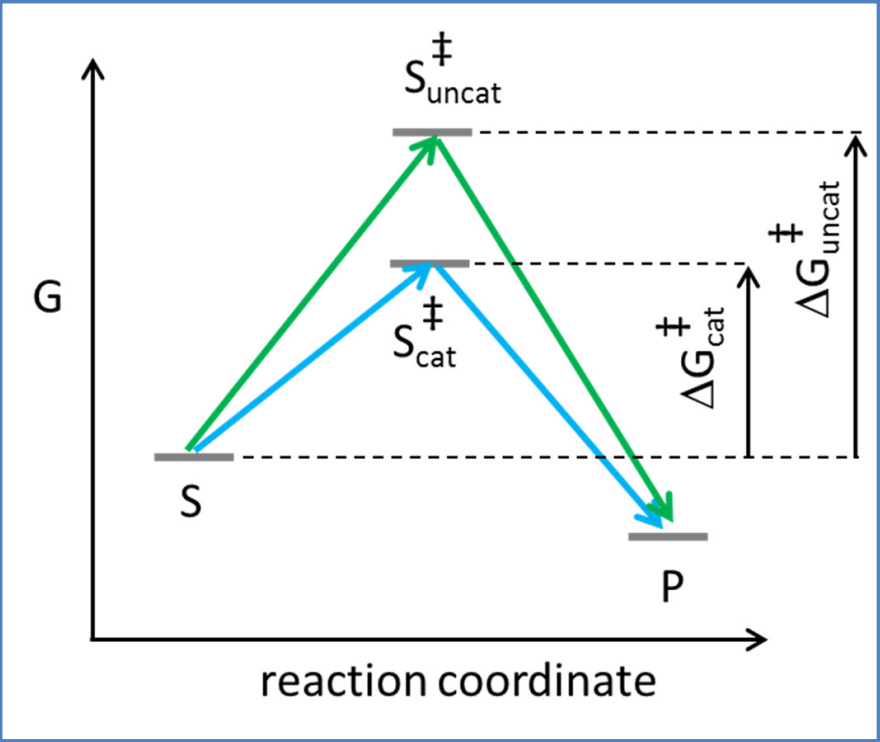
\includegraphics[scale = 0.5]{Catalysis .png}
\end{center}
\newpage


The surface configuration of the enyzme is complimentary to the unstable molecule with only transient existence (intermediate state), 
or the "activated complex" for the reaction that is catalyzed by that reaction. The enzyme would show attraction for the substrate, which 
would become attached to it in its active surface region. The substrate would be strained, and typically deform into the configuration of 
the activated complex. The activated complex then reassumes the original configuration or turns into the product. 

\begin{center}
    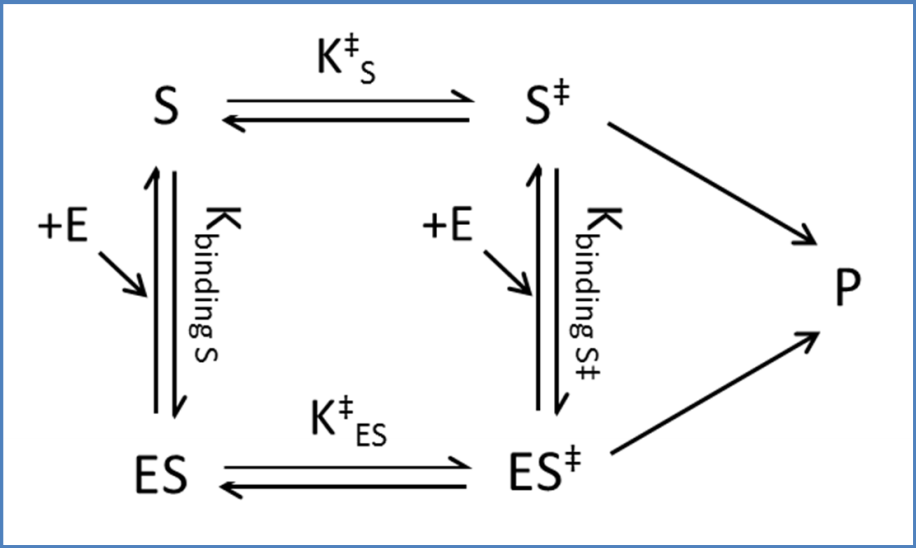
\includegraphics[scale = 0.5]{Kbinding.png}
\end{center}

We can relate the binding events in the presence of an enzyme to the formation of the transition state. The reactions on the \textbf{top} describe the reaction in 
the \textbf{absence} of the enzyme. The reactions on the bottom describe reaction with enzyme. The ratio between the rate constants with and without enzymes is: 

\begin{equation*}
    \frac{k_{cat}}{k_{uncat}} = \frac{K^{\ddagger}_{ES}}{K^{\ddagger}_S}
\end{equation*}

By providing a binding surface that is complimentary to the transition state form for substrate, the equilibrium constant for reaching the transition state
is increased by mass action $\rightarrow$ reaction is sped up. 

The ratio for how much a reaction is sped up is: 

\begin{equation*}
    \frac{k_{cat}}{k_{uncat}} = \frac{K^{\ddagger}_{ES}}{K^{\ddagger}_S} = \frac{K_{binding S \ddagger}}{K_{binding S}}
\end{equation*}

By this equation: the enzyme speeds up its reaction by binding exceptionally tightly to the transition state form of the substrate. 
This is what lowers the free energy of the transition state.

\newpage

\subsection*{Practical Consequences of Enzymes Binding Tightly to the Transition State}

\subsubsection*{Transition state analogues as enzyme inhibitors}
If an enzyme speeds up a reaction by a factor of 1000, then by the math above, the enzyme binds the transition state form of the substrate ($S\ddagger$) 
more tightly than it binds the substrate. 

A drug molecule that looks like the $S\ddagger$ will bind tightly to the eznyme and thus act as an inhibitor. The main challenge is that the transition state is unstable. 
The main goal is to find a compound that looks as similar to the transition state, but is still stable. 

\subsubsection*{Creating new enzymes from a natural antibody repertoire}
The goal was to create novel enzymes that would catalyze useful chemical types of reactions that no natural enzymes had evolved to carry out. 

If you can find an antibody sequence with a high affinity for the transition state of a desirable reaction, then you have found an enzyme for that reaction. 

\subsubsection*{Computational Enzyme Design}
Instead of designing a novel protein from scratch, take a natural protein that has a surface cleft suitable for binding a compound of about the right size. 
Then modify the amino acid sequence mainly within the binding site cleft. No need to create transition state analogs, and instead only requires an accurate model 
for what the transition state is likely to look like. Computer programs can then design reasonable models of transition states. 

The most challenging part is designing amino acid changes into a protein so that the TS is tightly bound. One issue concerns the calculation of free energies for large systems like 
proteins and their complexes. 

Changing amino acid sequences can also cause loss of stability and aggregation, or make alternate (non-native) configurations more stable than the intended structure. 

\newpage

\subsection*{Kinetic Parameters of Natural Enzymes}
Part of the complexity concerns the saturation behavior of enzyme kinetics. 

\begin{equation*}
    v = \frac{[E_{total}] k_{cat}[S]}{[S] + K_M}
\end{equation*}

An enzyme that has a high $k_{cat}$ may not be great if it does not bind substrate well (i.e. if $K_M$ is high). 
The best conditions is to have \textbf{high} $k_{cat}$ and \textbf{low} $K_M$. 

The ratio of $\frac{k_{cat}}{K_M}$ is considered the general measure of efficiency of an enzyme. $k_{cat}$ is the maximum velocity at any substrate concentration. 
$\frac{k_{cat}}{K_M}$ is the slope of the velocity curve in its linear region well below saturation. We are evaluating the standard Michaelis-Menten velocity equation (above) at $[S] \ll K_M$. 

Typically, $K_M$ values exhibited by natural enzymes tend to be roughly in the same range as natural cellular concentration of the substrate on which they operate. 

\newpage
\section*{Chapter 17: Introduction to Biochemical Spectroscopy}

\subsection*{Energy Transitions}

From quantum mechanics, we know that molecules can exist only in discrete energy states. Transitions between one energy state and another 
can be driven by absorption/emission of electormagnetic radiation (photons) if the energy of the phton matches the energy difference of the 
transition. 

The relationship between  frequency or wavelength of radiation and energy is: 

\begin{equation*}
    E = hv = \frac{hc}{\lambda}
\end{equation*}

\begin{center}
    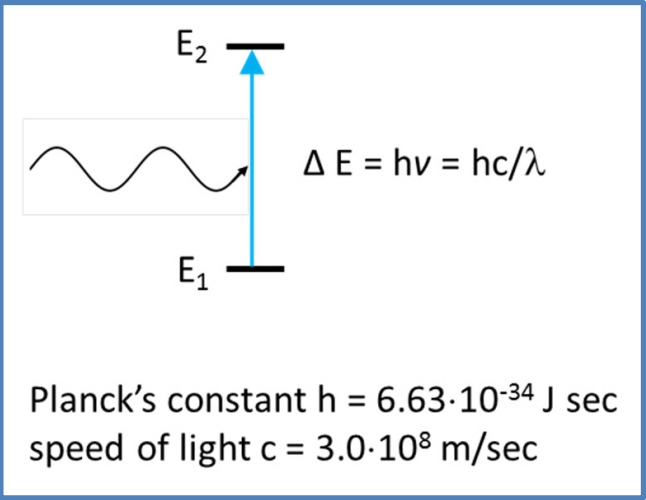
\includegraphics[scale = 0.75]{energy transitions.png}
\end{center}

Simple molecules (like single atoms) show very sharp absorption and emission bands. 

They only undergo transitions at very narrow wavelengths $\longrightarrow$ \textbf{Rydberg Series}. 

However, complex molecules have complex spectra. Presence of multiple atoms in a molecule introduces
dependence of energy on nuclear positions. 

Nuclear motions give rise to vibrational energy states. The energy differences in vibrational states is much 
smaller than those between electronic states. Within vibrational states are even smaller rotational states. 
This heirarchal level of complexity allows for a huge number of transitions with closely spcaed energies. 

As a result, absorption and emission spectra for larger molecules are coplex and more continuous in nature rather than discrete. 

\begin{center}
    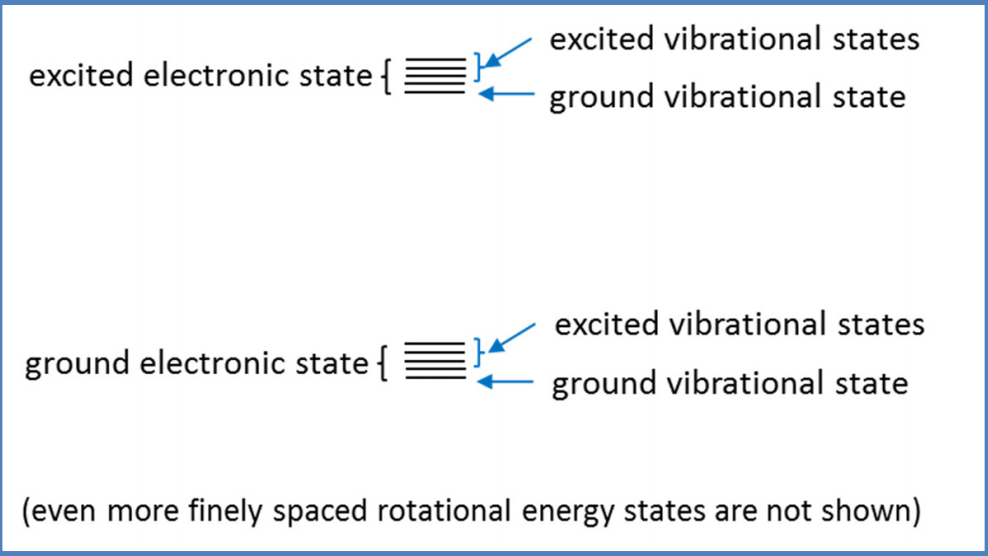
\includegraphics[scale = 0.75]{energy states.png}
\end{center}

Consider an energy associated with wavelength of 400 nm in the violet region of the visible spectrum.
\begin{equation*}
    E = hv = \frac{hc}{\lambda} = 4.1 \times 10^{-21} J 
\end{equation*}
This is equivalent to about 120$K_B$T. According to the Boltzmann equation ($e^{-\frac{E}{K_BT}}$), the probability of a molecule being in this excited state 
rather than ground state is basically zero. 

Repeat this for a typical vibrational transition. Consider a typical stretch where $\lambda = 1.9$  $\mu M.$
The energy is about \(1.4 \times 10^{-19} J \) or about 25 $K_BT$. The probability is much higher here. 

\textbf{Conclusion:} At ordinary temperatures and unless otherwise excited, molecules almost exclusively populate the lowest vibrational state of the lowest electronic state. 
\textbf{A high probability transition requires the initial energy state to be well-populated}.

\subsection*{Fluorescence}

Our analysis from above tells us that an absoprtion transition usually happens from the ground vibrational state 
of the ground electronic state. 

The next question is: to what higher electronic energ state is a molecule likely to be excited by absorption. 

\textbf{General Idea:} Lowest energy nuclear positions for a molecule are slihgtly different for different eletronic states. 
\newpage

\begin{center}
    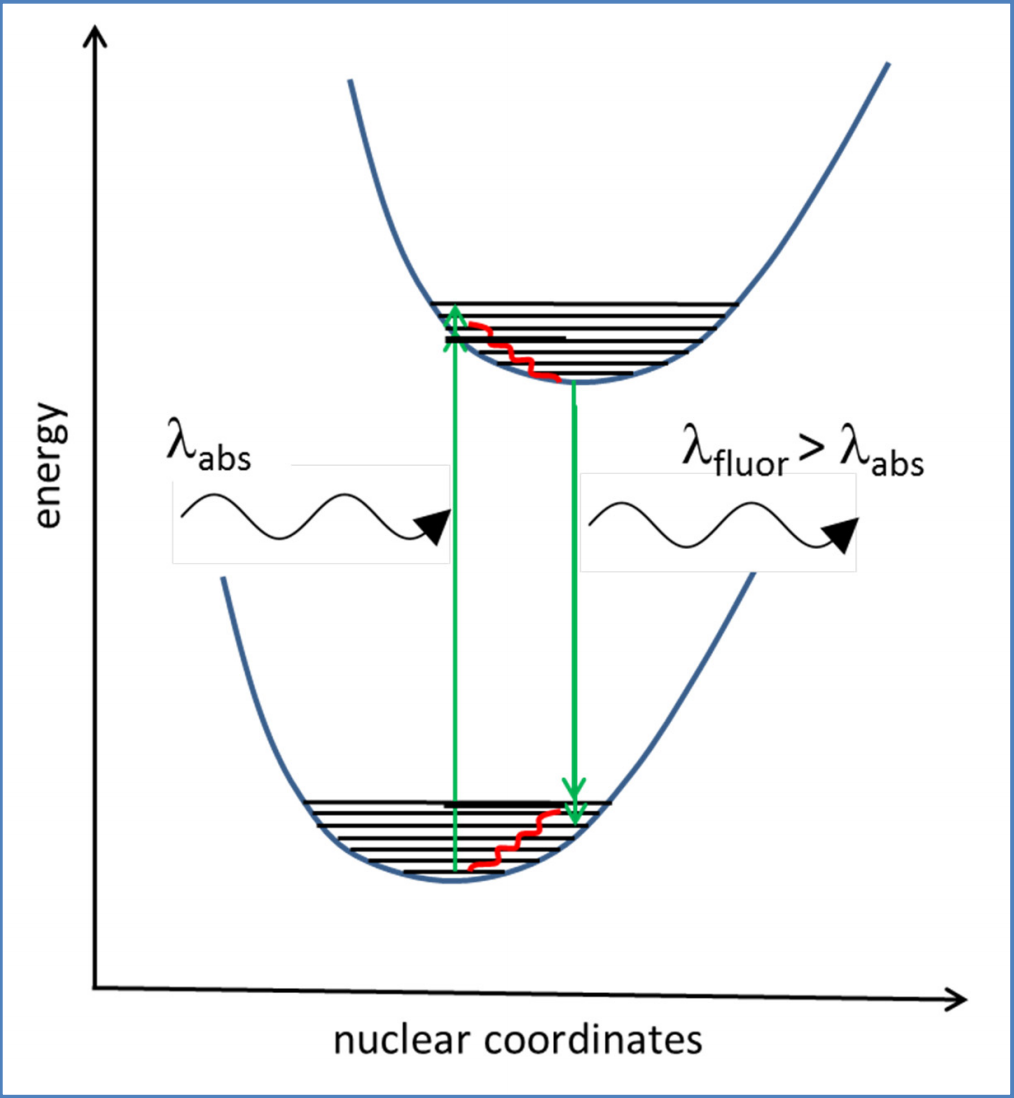
\includegraphics[scale = 0.50]{fluorescence.png}
\end{center}

Consider the image below. The two black currves indicate the classical energy of a molecule as a function of its nuclear positions in two different
energy states. The minimum energies occur at slighly different nuclear positions. These are illustrated by the green lines coming from the lowest horiziontal line
in each curve. 

The width of the lines illustrate the range of nuclear positions that are allowed in each vibrational state. 
The timescale for photon absorption is much shorter than the timescale for nuclear motions. This means that electronic transitions happen 
"vertically" in the disgram shown. 

$\underline{The \text{ } Franck-Condon \text{ } Principle:}$ When a molecule is undergoing an electronic transition (like ionization), the nuclear configuration of the molecule experiences no significant change.

Nuclei are much bigger than electrons, and electronic transitions happen faster than the nuclei can respond. When the nuclei finally realigns itself
with the new electronic configuration, it then undergoes a \textbf{vibration}. 

If an electronic transition must occur without appreciable movement of nuclei, then it must occur to a vibrational state for which initial nuclear positions are allowable. 

After excitation, according to the Boltzmann equation, a molecule must return to the ground state. This can occur with the emission of a photon. This is known as 
\textbf{fluorescence.} The timescale for fluorescence is typically in the \( 10^{-5} - 10^{-8} sec \) range. 
This is long enough for thermal vibrations and collisions to allow the molecule to descent to lower vibrational states within excited electronic state, before returning 
to the ground electronic state. 

The \textbf{key consequence} is that the fluorescence emission spectrum for a molecule is shifted to lower energy and longer wavelength compared to absoprtion spectrum.
This is known as \textbf{Stoke's Shift}. 

\begin{center}
    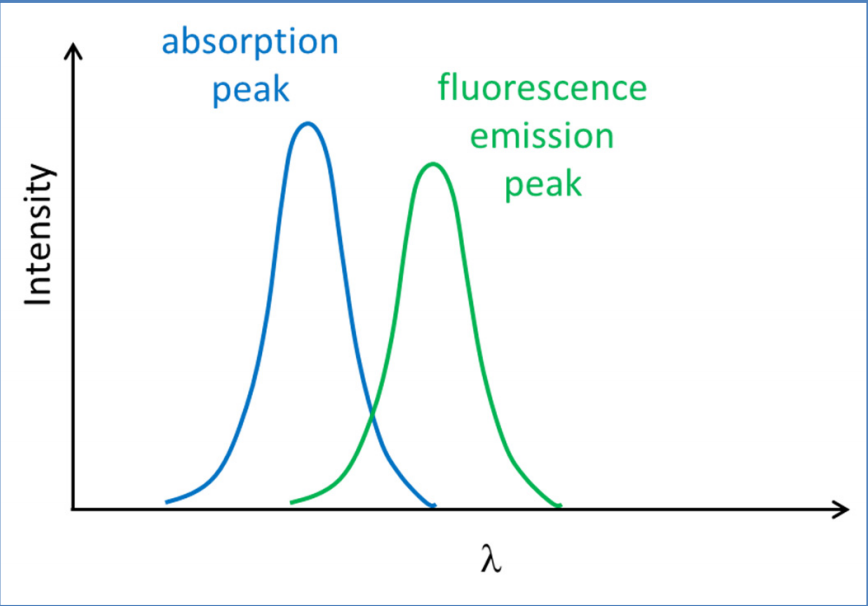
\includegraphics[scale = 0.50]{stokes shift.png}
\end{center}

\subsubsection*{Uses and Advantageous Properties of Fluorescence}
Fluorescence offers a high degree of sensitivity for detecing and measuring concentrations of specific molecules. 
The high sensitivity of fluorescence comes from two factors. 

First is the shift in wavelength from incident wavelength to emission wavelength. In an absorption experiment involving 
dilute molecule, you must analyze a small difference between two large numbers: the number of photons transmitted by a blank compared to 
number transmitted by the sample. 

But, in a fluorescence experiment, the change in wavelength makes it possible to analyze the number of emitted photons without interference from 
transmitted photons, which have the same wavelength as the incident light. 

\newpage

This requires a second monochromator placed between the sample and the detector, and a first monochromator is required between the light source and the sample. 
Extra level of sensitivity comes from the ability to monitor fluorescence in a direction different from the path of the transmitted beam. Scatted photons travel in all directions
including the same path as fluorescent photons. But, since their wavelength is the same as the incident wavelength, they are distinguishable. 

\begin{center}
    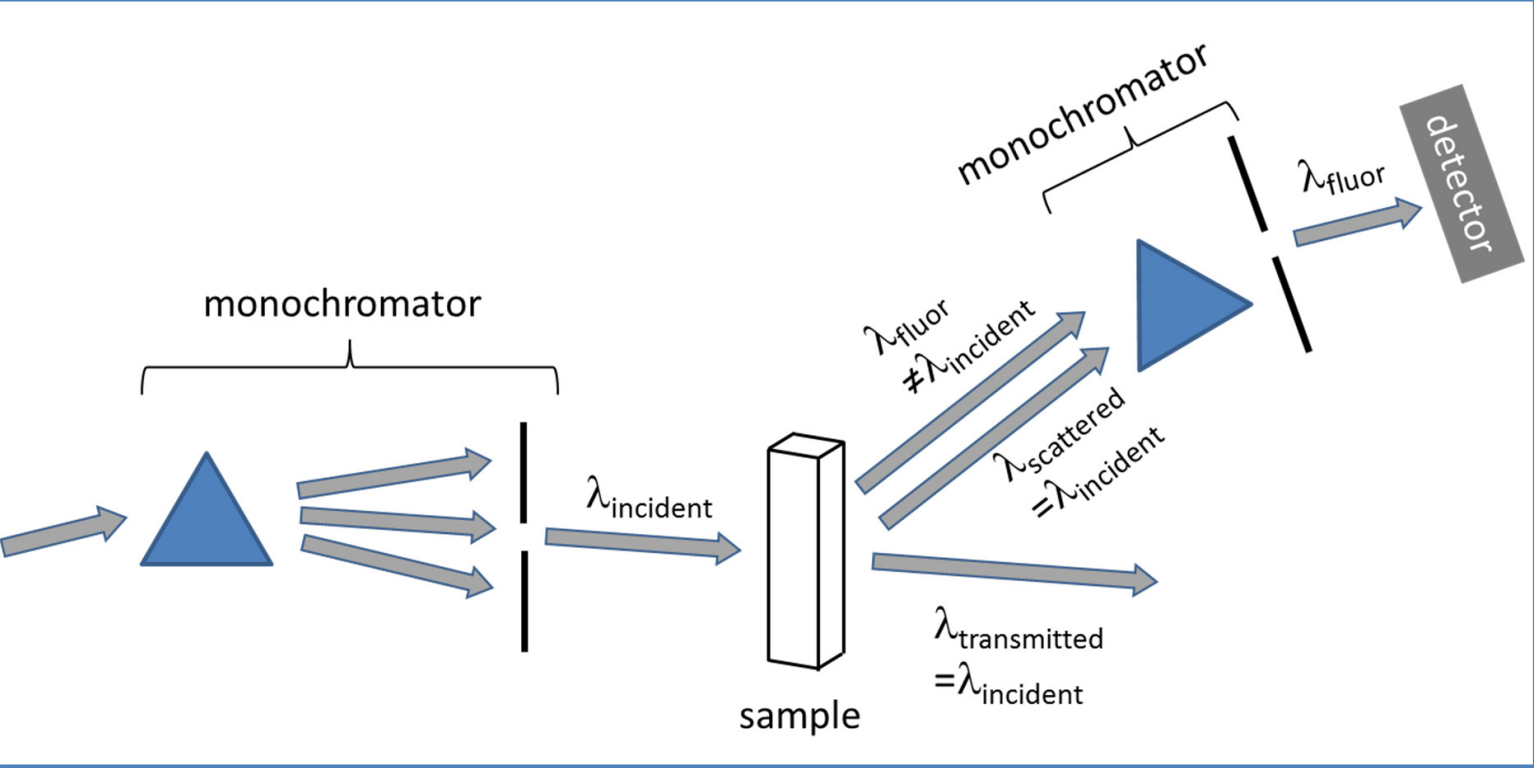
\includegraphics[scale = 0.35]{fluorescence experiment.png}
\end{center}

Proteins typically have natural fluorescence owing to the presence of tryptophan amino acids. A particularly useful feature of fluorescence is its 
sensitivity to chemical environment. The greater sensitivity to environment for fluorescence compared to absorbance relates in part to the longer time 
scale of fluorescence. In general, increased flexibility and enviornmental polarity lead to lower fluorescent intensity. The peak emission wavelength can also 
be affected. 

For example, fluorescence of tryptophan increases by a factor of 4 in a low polarity solvent (like DMSO, $\epsilon$ = 35) compared to water ($\epsilon$ = 80). 
Tryptophan resides almost always become less flexible and more rigidly held in the folded state of a protein, thus leading to higher fluorescence. 

\newpage

\subsection*{Kinetics of Fluorescence and competing routes for return to ground state}

 After a molecule has been driven to an excited state by absorbing a photon, there are several 
 routes it can take to return to ground state. The relative rates of these processes relates directly to which 
 pathways dominate for a given molecule. 

 If the rate constant for fluorescent emission is higher than the rate constants for other processes, then most 
 of the excited molecules will return to the ground state by way of fluorescent emission. 

 \begin{center}
    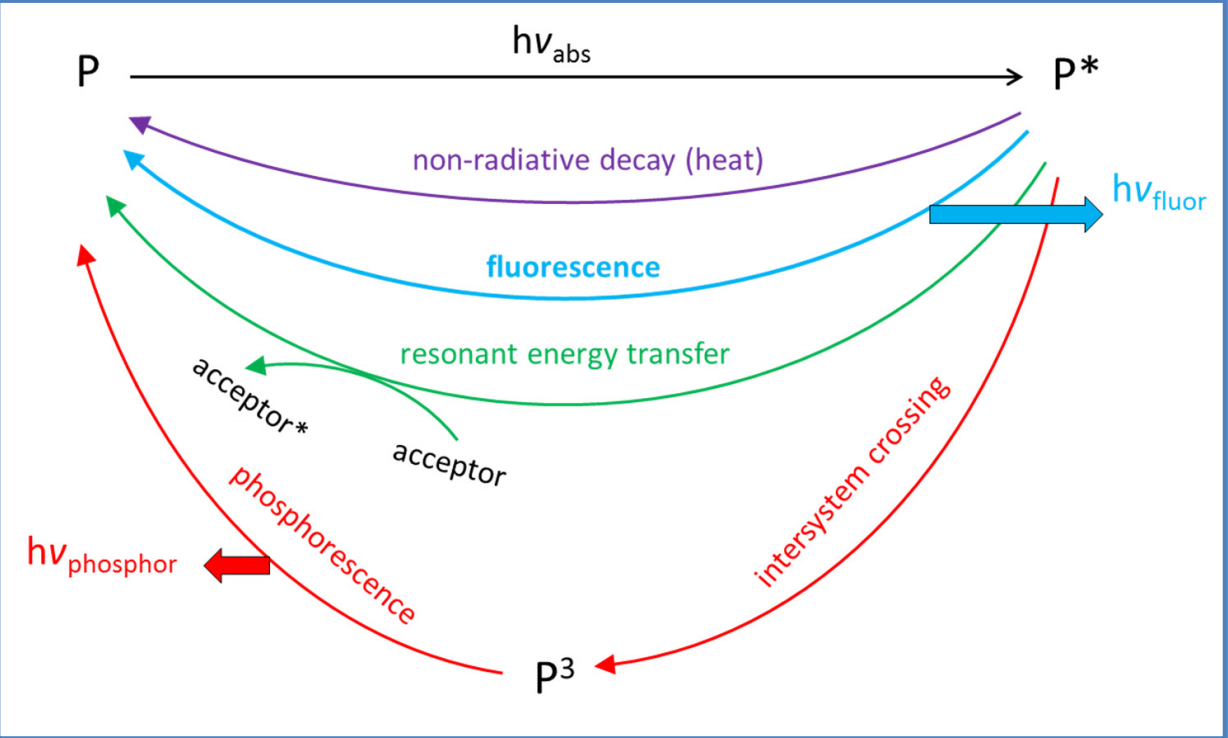
\includegraphics[scale = 0.5]{ground states.png}
 \end{center}

 A number of phenomena affect fluorescence, including chemical environment, so fluorescence can be used to monitor
 various events that alter the environment of a fluorophore in solution. 

 We can lump together the various non-fluorescent pathways for return to ground state under a single rate constant, \textbf{$k_{other}$}. 
 Various events can then be analyzed in terms of the effects they have on the relative rates of $k_{fluor}$ and $k_{other}$. 

 With respect to kinetic treatments, fluorescence experiments can be of two essentially different types: 
 
 1. Under continuous illumination where steady state behavior is assumed

 2. Following a brief pulse of incident light, after which time-dependent measurements are made.

 \begin{center}
    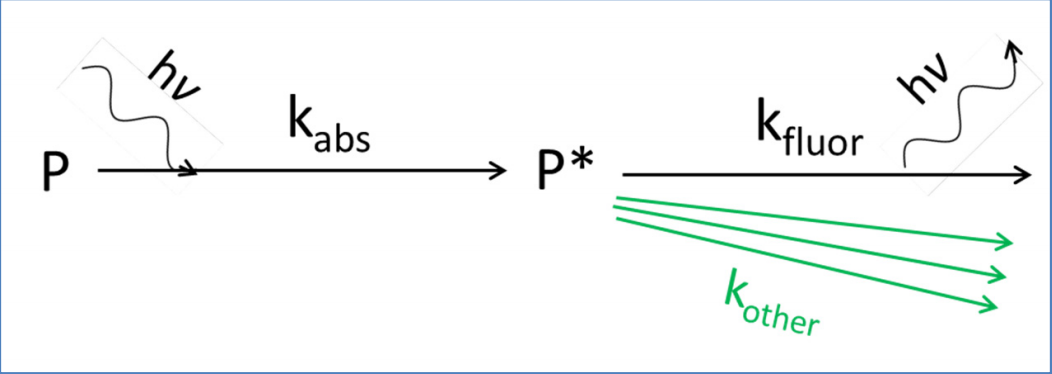
\includegraphics[scale = 0.5]{fluorescent experiment.png}
 \end{center}

 \subsubsection*{Constant Illumination}
 Under constant illumination, the concentration of the excited fluorophore ($P^*$) is not changing. 
 Setting $\frac{d[P^*]}{dt} = 0$: 

 \begin{align*}
    \frac{d[P^*]}{dt} &= 0 \\ \\ 
    &= k_{abs}[P] - (k_{fluor} + k_{other}[P^*])
 \end{align*}

 Rearranging to obtain an expression for $[P^*]$: 

 \begin{equation*}
    [P^*] = \frac{k_{abs}[P]}{k_{fluor} + k_{other}}
 \end{equation*}

 Then, the fluorescent intensity $I_{fluor}$ is given by: 

 \begin{align*}
    I_{fluor} &= k_{fluor}[P^*] \\ \\
    &= \frac{k_{abs}[P] * k_{fluor}}{k_{fluor} + k_{other}}
 \end{align*}

 Since the rate of photon absorption is $k_{abs}$[P], the ratio of number of phtoons emitted to the number absorbed - a fractional quantity known as the \textbf{quantum yield Q}  - 
 is given by: 

 \begin{equation*}
    Q = \frac{k_{fluor}}{k_{fluor} + k_{other}}
 \end{equation*}

 The quantum yield and intensity of fluorescence observed under constant illumination is decreased by events in solution that increase the rates of non-fluorescent "other" pathways
 for return to ground state. 

 \begin{center}
    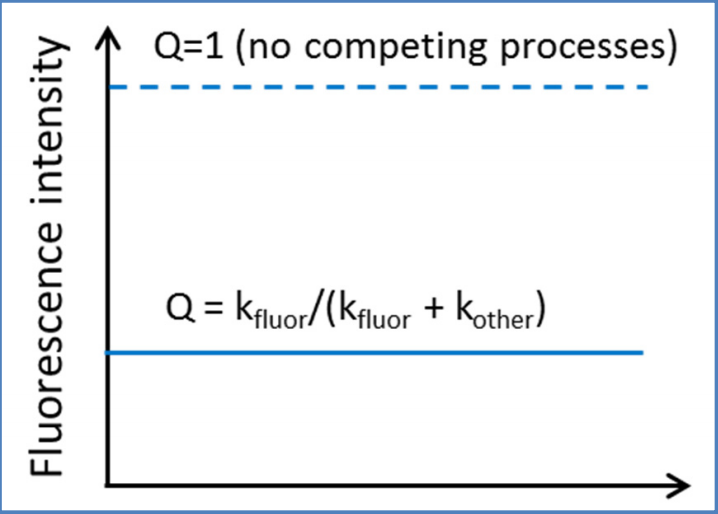
\includegraphics{quantum.png}
 \end{center}

 An example is shown above. The binding of a fluorescent molecule to a protein would decrease the non-fluorescent pathways by reducing mobility of the fluorophore and thereby increase the 
 quantum yield along with the steady state fluorescence intensity. 

 \subsubsection*{Time-resolved Fluorescence}
 An excitation pulse can be applied and the fluorescence intensity (which must decay back to zero) can be monitored over time. The same kinetic scheme as above can be used if 
 we remove the continuous absorption event. This becomes a simple case of exponential decay with a total rate constant of $k_{fluor} + k_{other}$ and a decay time of: 

 \begin{equation*}
    \tau = \frac{1}{k_{fluor}}+ k_{other}
 \end{equation*}

\newpage

\section*{Chapter 18: Special Topics in Biochemical Spectroscopy}



\end{document}
